\documentclass[10.5pt]{article}

\usepackage{amsmath,amssymb,amsthm}
\usepackage{listings}
\usepackage{graphicx}
\usepackage[shortlabels]{enumitem}
\usepackage{tikz}
\usepackage[margin=1in]{geometry}
\usepackage{fancyhdr}
\usepackage{epsfig} %% for loading postscript figures
\usepackage{amsmath}
\usepackage{float}
\usepackage{amssymb}
\usepackage{caption}
\usepackage{subfigure}
\usepackage{graphics}
\usepackage{titlesec}
\usepackage{mathrsfs}
\usepackage{amsfonts}
\usepackage{indentfirst}
\usepackage{color}
\usepackage{algorithm}
\usepackage{algorithmicx}
\usepackage{algpseudocode}
\usepackage{tikz-qtree}
\renewcommand{\baselinestretch}{1.2}%Adjust Line Spacing
%\geometry{left=2.0cm,right=2.0cm,top=2.0cm,bottom=2.0cm}% Adjust Margins of the File
\usetikzlibrary{graphs}
\tikzset{every tree node/.style={minimum width=2em,draw,circle},
	blank/.style={draw=none},
	edge from parent/.style=
	{draw,edge from parent path={(\tikzparentnode) -- (\tikzchildnode)}},
	level distance=1.2cm}
\setlength{\parindent}{0pt}
%\setlength{\parskip}{5pt plus 1pt}
\setlength{\headheight}{13.6pt}
\newcommand\question[2]{\vspace{.25in}\hrule\textbf{#1: #2}\vspace{.5em}\hrule\vspace{.10in}}
\renewcommand\part[1]{\vspace{.10in}\textbf{(#1)}}
%\newcommand\algorithm{\vspace{.10in}\textbf{Algorithm: }}
\newcommand\correctness{\vspace{.10in}\textbf{Correctness: }}
\newcommand\runtime{\vspace{.10in}\textbf{Running time: }}
\pagestyle{fancyplain}
% Create horizontal rule command with an argument of height
\newcommand{\horrule}[1]{\rule{\linewidth}{#1}}



% Set the title here
\title{
	\normalfont \normalsize
	\textsc{ShanghaiTech University} \\ [25pt]
	\horrule{0.5pt} \\[0.4cm] % Thin top horizontal rule
	\huge CS101 Algorithms and Data Structures\\ % The assignment title
	\LARGE Fall 2021\\
	\LARGE Homework 6\\
	\horrule{2pt} \\[0.5cm] % Thick bottom horizontal rule
}
% wrong usage of \author, never mind
\author{}
\date{Due date: 23:59, November 7, 2021}

% set the header and footer
\pagestyle{fancy}
\lhead{CS101 Algorithms and Data Structures}
\chead{Homework 6}
\rhead{Due date: 23:59, Nov. 7, 2021}
\cfoot{\thepage}
\renewcommand{\headrulewidth}{0.4pt}
\newtheorem{Q}{Question}
% special settings for the first page
\fancypagestyle{firstpage}
{
	\renewcommand{\headrulewidth}{0pt}
	\fancyhf{}
	\fancyfoot[C]{\thepage}
}

% Add the support for auto numbering
% use \problem{title} or \problem[number]{title} to add a new problem
% also \subproblem is supported, just use it like \subsection
\newcounter{ProblemCounter}
\newcounter{oldvalue}
\newcommand{\problem}[2][-1]{
	\setcounter{oldvalue}{\value{secnumdepth}}
	\setcounter{secnumdepth}{0}
	\ifnum#1>-1
	\setcounter{ProblemCounter}{0}
	\else
	\stepcounter{ProblemCounter}
	\fi
	\section{Problem \arabic{ProblemCounter}: #2}
	\setcounter{secnumdepth}{\value{oldvalue}}
}
\newcommand{\subproblem}[1]{
	\setcounter{oldvalue}{\value{section}}
	\setcounter{section}{\value{ProblemCounter}}
	\subsection{#1}
	\setcounter{section}{\value{oldvalue}}
}

% \setmonofont{Consolas}
\definecolor{blve}{rgb}{0.3372549 , 0.61176471, 0.83921569}
\definecolor{gr33n}{rgb}{0.29019608, 0.7372549 , 0.64705882}
\makeatletter
\lst@InstallKeywords k{class}{classstyle}\slshape{classstyle}{}ld
\makeatother
\lstset{language=C++,
	basicstyle=\ttfamily,
	keywordstyle=\color{blve}\ttfamily,
	stringstyle=\color{red}\ttfamily,
	commentstyle=\color{magenta}\ttfamily,
	morecomment=[l][\color{magenta}]{\#},
	classstyle = \bfseries\color{gr33n}, 
	tabsize=4
}
\lstset{basicstyle=\ttfamily}
\begin{document}
	
	\maketitle
	\thispagestyle{firstpage}
	%\newpage
	\vspace{3ex}
	
	\begin{enumerate}
		\item Please write your solutions in English. 
		
		\item Submit your solutions to gradescope.com.  
		
		\item Set your FULL NAME to your Chinese name and your STUDENT ID correctly in Account Settings. 
		
		\item If you want to submit a handwritten version, scan it clearly. Camscanner is recommended. 
		
		\item When submitting, match your solutions to the according problem numbers correctly. 
		
		\item No late submission will be accepted.
		
		\item Violations to any of the above may result in zero grade. 
	\end{enumerate}
	\newpage


\question{1}{(12') Multiple Choices}
	Each question has one or more correct answer(s). Select all the correct answer(s). For each question, you get $0$ point if you select one or more wrong answers, but you get $1$ point if you select a non-empty subset of the correct answers.\\
\textit{Note that you should write you answers of section 1 in the table below.}

\begin{table}[htbp]
	\begin{tabular}{|p{2cm}|p{2cm}|p{2cm}|p{2cm}|p{2cm}|p{2cm}|}
		\hline 
		Question 1 & Question 2 & Question 3 & Question 4 & Question 5 & Question 6  \\ 
		\hline 
		C & B D & B D & A D & A & A C \\ 
		\hline 
	\end{tabular} 
\end{table}

\begin{Q}
	Which of the followings are true? 
	\begin{enumerate}[(A)]
		\item For a min-heap, in-order traversal gives the elements in ascending order.
		\item For a min-heap, pre-order traversal gives the elements in ascending order.
		\item For a BST, in-order traversal gives the elements in ascending order.
		\item For a BST, pre-order traversal gives the elements in ascending order.
	\end{enumerate}
\end{Q}

\begin{Q}
	For a Binary Search Tree (BST), which of the followings are true?
	
	\begin{enumerate}[(A)]
		\item If we erase the root node with two children, then it will be replaced by the maximum object in its right sub-tree.
		\item The cost for erasing the root node who has two children is $O(n)$. 
		\item In a BST with N nodes, it always takes $O(\log N)$ to search for an specific element.
		\item For a BST, the newly inserted node will always be a leaf node.
	\end{enumerate}
\end{Q}


\begin{Q}
	Suppose we want to use Huffman Coding Algorithm to encode a piece of text made of characters. Which of the following statements are true?
	\begin{enumerate}[(A)]
		\item Huffman Coding Algorithm will  compress the text data with some information loss.
		\item The construction of binary Huffman Coding Tree using priority queue has time complexity $O(nlogn)$, where $n$ is the size of the character set of the text.
		\item When inserting nodes into the priority queue, the higher the occurrence/frequency, the higher the priority in the queue.
		\item The Huffman codes obtained must satisfy prefix-property, that is, no code is a prefix of another code.
	\end{enumerate}
\end{Q}

	\begin{Q}
		Which of the following statements are true for an AVL-tree?
		\begin{enumerate}[(A)]
			\item Inserting an item can unbalance non-consecutive nodes on the path from the root to the inserted item before the restructuring.
			\item Inserting an item can cause at most one node imbalanced before the restructuring.
			\item Removing an item in leaf nodes can cause at most one node imbalanced before the restructuring.
			\item Only at most one node-restructuring has to be performed after inserting an item.
		\end{enumerate}
	\end{Q}
	
	\begin{Q}
		Consider an AVL tree whose height is h, which of the following are true?
		\begin{enumerate}[(A)]
			\item This tree contains $\Omega(\alpha^h)$ nodes, where $\alpha = \dfrac{1+\sqrt{5}}{2}$.
			\item This tree contains $\Theta(2^h)$ nodes.
			\item This tree contains $O(h)$ nodes in the worst case.
			\item None of the above.
		\end{enumerate}
	\end{Q}
	
	
	\begin{Q}
		Which of the following is TRUE?
		\begin{enumerate}
			\item[(A)] The cost of searching an AVL tree is $O(\log n)$ but that of a binary search tree is $O(n)$
			\item[(B)] The cost of searching an AVL tree is $O(\log n)$ but that of a complete binary tree is $O(n \log n)$
			\item[(C)] The cost of searching a binary search tree with height h is $O(h)$ but that of an AVL tree is $O(\log n)$
			\item[(D)] The cost of searching an AVL tree is $O(n log n)$ but that of a binary search tree is $O(n)$
		\end{enumerate}
	\end{Q}
\vspace{0.5cm}
\pagebreak

\question{2}{(3'+3'+2'+3') BST and AVL Tree}
\begin{Q}
Draw a valid BST of minimum height containing the keys 1, 2, 4, 6, 7, 9, 10.
\vspace{1em}\\
\textbf{Solution:}\\
\begin{center}
	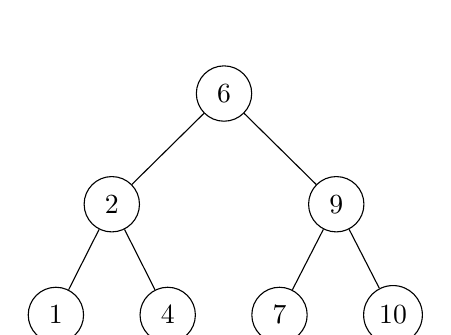
\begin{tikzpicture}[sibling distance=20pt, level distance=40pt]
		\Tree 
		[.6
			[.2 1 4
			]
			[.9 7 10
			]
		]
	\end{tikzpicture}
\end{center}
\end{Q}


	
\begin{Q}\text{}\\
	\begin{enumerate}[(1)]
		\item 
		Given an empty AVL tree, insert the sequence of integers $15, 20, 23, 10, 13, 7, 30, 25$ from left to right into the AVL tree. Draw the final AVL tree.\\
		\textbf{Solution:}\\
		\begin{center}
			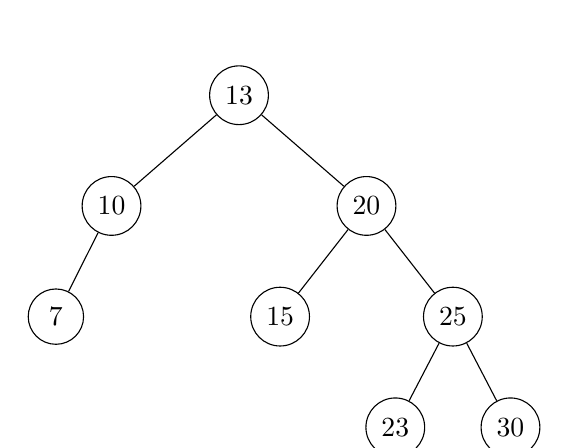
\begin{tikzpicture}[sibling distance=20pt, level distance=40pt]
				\Tree
				[.13
					[.10 7 \edge[blank];\node[blank]{};
					]
					[.20 15
					 [.25 23 30
					 ]
					]
				]
			\end{tikzpicture}
		\end{center}
		\item
		For the final AVL tree in the question (1), delete $7$. Draw the AVL tree after deletion.\\
		\textbf{Solution:}\\
		\begin{center}
			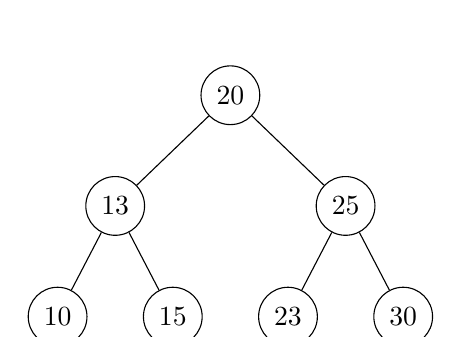
\begin{tikzpicture}[sibling distance=20pt, level distance=40pt]
				\Tree
				[.20
					[.13 10 15
					]
					[.25 23 30
					]
				]
			\end{tikzpicture}
		\end{center}
		\item
		For an AVL tree, define D = the number of left children - the number of right children,  for the root. Then what is the maximum of D for an AVL tree with height n ?\\
		\textbf{Solution:}\\
		\textup{The maximum of $D$ should be the maximum number of the nodes in the left subtree minus the minimum number of the nodes in the right tree.}
		$$
			D_{max} = L_M - R_m
		$$
		\textup{Therefore, the height of the left subtree shoud be $n - 1$ and the height of the right substree shuold be $n - 2$. The number of the nodes in the left substree is maximized when the left substree is a perfect tree. Then we have}
		$$
		L_M = 2^n - 1
		$$ 
		\textup{The right subtree should also be an AVL tree. The minimum number of the nodes in the right substree is the minimum number of the nodes in an AVL tree with height $n - 2$. Let the minumber number of the nodes in an AVL tree with given heght $h$ be denoted as $F(h)$. Each AVL tree can be seperate into left subtree, right subtree and the root. Both the left substree and the right subtree also have minimal number of nodes. One of the height of the subtree should be $h - 1$ and the other should be $h - 2$. Therefore, we have:}
		$$
		\begin{cases}
			F(h) = 1 + F(h - 1) + F(h - 2) & (*)\\
			F(0) = 1 \\
			F(1) = 2 
		\end{cases}
		$$
		\textup{The $(*)$ can also be represented as follows:}
		$$
		F(h) + 1 = \left[F(h - 1) + 1\right] + \left[F(h - 2) + 1\right]
		$$
		\textup{Let $G(h) = F(h) + 1$}\\
		$$
		\begin{cases}
			G(h) = G(h - 1) + G(h - 2)\\
			G(0) = 2\\
			G(1) = 3\\
		\end{cases}
		$$
		\textup{The chacracteristic funciton is}
		\begin{align*}
			x^2& = x + 1\\
			x_1 &= \frac{1 + \sqrt{5}}{2}\\ 
			x_2 &= \frac{1 - \sqrt{5}}{2}
		\end{align*}
		\textup{Then we have}
		\begin{align*}
			G(h) &= c_1(x_1)^h + c_2(x_2)^h\\
			G(0) &= c_1 + c_2 = 2\\
			G(1) &= \frac{1+\sqrt 5}{2}c_1 + \frac{1-\sqrt 5}{2} = 3\\
			c_1&=\frac{5+2\sqrt{5}}{5},\\ c_2 &=\frac{5-2\sqrt 5}{5}
		\end{align*}
		\textup{Therefore}
		\begin{align*}
			G(h) &= \frac{5+2\sqrt{5}}{5}\cdot\left(\frac{1 + \sqrt{5}}{2}\right)^h + \frac{5-2\sqrt 5}{5}\cdot\left(\frac{1 - \sqrt{5}}{2}\right)^h\\
			F(h) &= \frac{5+2\sqrt{5}}{5}\cdot\left(\frac{1 + \sqrt{5}}{2}\right)^h + \frac{5-2\sqrt 5}{5}\cdot\left(\frac{1 - \sqrt{5}}{2}\right)^h - 1
		\end{align*}
		\textup{Then we can calculate $R_m$}
		$$
		R_m = F(n - 2) = \frac{5+2\sqrt{5}}{5}\cdot\left(\frac{1 + \sqrt{5}}{2}\right)^{(n - 2)} + \frac{5-2\sqrt 5}{5}\cdot\left(\frac{1 - \sqrt{5}}{2}\right)^{(n - 2)} - 1 = G(n - 2) - 1
		$$
		\textup{Hence,}
		\begin{align*}
			D_{max} & = L_M - R_m\\
				&= (2^n - 1) - (G(n - 2) - 1)\\
				&= 2^n - G(n - 2)\\
				&= 2^n - \frac{5+2\sqrt{5}}{5}\cdot\left(\frac{1 + \sqrt{5}}{2}\right)^{(n - 2)} - \frac{5-2\sqrt 5}{5}\cdot\left(\frac{1 - \sqrt{5}}{2}\right)^{(n - 2)}
		\end{align*}
	\end{enumerate}
\end{Q}

\newpage
\question{3}{(3'+3') Huffman Coding}
	
    After you compress a text file using Huffman Coding Algorithm, you accidentally spilled some ink on it and you found that one word becomes unrecognizable. Now, you need to recover that word given the following information:\\
    \textbf{Huffman-Encoded sequence of that word: } \\
    000101001110110100\\
    \textbf{Frequency table that stores the frequency of some characters: }
    \begin{table}[!hbtp]
    \begin{tabular}{|l|l|l|l|l|l|l|l|l|}
    \hline
    characters & a & b & e & g & l & o & r \\ \hline
    frequency  & 2 & 3 & 3 & 4 & 1 & 4 & 2 \\ \hline
    \end{tabular}
    \end{table}
	\begin{Q} Please construct the binary Huffman Coding Tree according to the given frequency table and draw the final tree below.\\
	Note: The initial priority queue is given as below. When popping nodes out of the priority queue, the nodes with the same frequency follows ``First In First Out".\\
	\end{Q}

		
	\begin{table}[!hbtp]
    \begin{tabular}{|l|l|l|l|l|l|l|}
    \hline
    \begin{tabular}[c]{@{}l@{}}l\\ 1\end{tabular} & \begin{tabular}[c]{@{}l@{}}a\\ 2\end{tabular} & \begin{tabular}[c]{@{}l@{}}r\\ 2\end{tabular} & \begin{tabular}[c]{@{}l@{}}b\\ 3\end{tabular} & \begin{tabular}[c]{@{}l@{}}e\\ 3\end{tabular} & \begin{tabular}[c]{@{}l@{}}g\\ 4\end{tabular} & \begin{tabular}[c]{@{}l@{}}o\\ 4\end{tabular} \\ \hline
    \end{tabular}
    \end{table}
	\textbf{Solution:}\\
	\begin{center}
		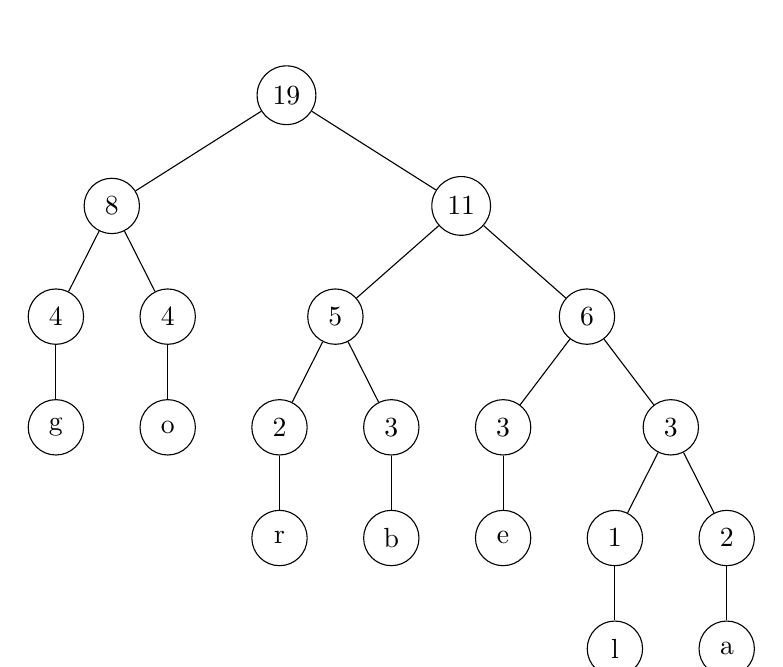
\begin{tikzpicture}[sibling distance=20pt, level distance=40pt]
			\Tree
			[.19
				[.8
					[.4 g
					]
					[.4 o
					]
				]
				[.11
					[.5
						[.2 r
						]
						[.3 b
						]
					]
					[.6
						[.3 e
						]
						[.3
							[.1 l
							]
							[.2 a
							]
						]
					]
				]
			]
		\end{tikzpicture}
	\end{center}
	\begin{Q} Now you can ``decompress" the encoded sequence and recover the original word you lost. Please write the original word below.\\
	\textbf{Solution:}\\
	\textup{googler}

	\end{Q}
	
	
\newpage

	
	\question{4}{(9')Only-child}
	We define that the node is only-child if its parent node only have one children(Note: The root does not qualify as an only child). And we define a function for any binary tree T : $OC(T)=$ the number of only-child node.
	
	
	\begin{Q}
		(3')Prove the conclusion that for any nonempty AVL tree T with n nodes, OC(T)$\leq\dfrac{1}{2}n$.\\
		\textbf{Solution:}\\
		\textup{\textbf{\underline{Claim:}} In an AVL tree, the only-child can only appear on the leaves.}\\
		\textup{\textbf{\underline{Proof:}} If an internal nodes $I$ is only-child, then his parent $P$ will be unbalanced. Since $I$ is only-child, then $P$ only has one child. Therefore, $P$ has a substree with height $0$. $I$ is internal node, it has at least one substree with height $h(h > 0)$. Therefore, the substree of $P$ containing $I$ has height $h + 1 > 1$, and the difference in height of the two subtree of $P$ is bigger than $1$. $P$ is unbalanced. Therefore, the only-child can only be leaf nodes.}\\
		\textup{Let $L$ be the number of leaf nodes, and $N$ be the be the number of the tree nodes.}\\
		\textup{\textbf{\underline{Claim:}} If a binary tree is not a full binary tree, $L \le \frac{N}{2}$.}\\
		\textup{\textbf{\underline{Proof:}} If the tree is a full binary tree, then $N = 2L - 1$, $L \le \frac{N + 1}{2}$. If the tree is not a full binary tree, we add $t(t>0)$ leave nodes to make it full and apply the relationship between leaves and nodes in full binary tree. $L' = L + t, N' = 2L' - 1, N = N' - t$. }
		\begin{align*}
			N &= N' - t\\
				&= 2L' - 1 - t\\
				&= 2L + 2t - t - 1\\
				&= 2L + t - 1 \ge 2L\\
			L &\le \frac{N}{2}
		\end{align*}
		\textup{Therefore, in a binary tree which is not a full binary tree, $L \le \frac{N}{2}$.}\\
		\textup{Next, we begin to prove that $OC(T)\le \frac12 n$.}\\
		\textup{We know that only-child node can only be leaf nodes in an AVL tree, and an only-child node can't have sibling node. If $T$ is not a full binary tree, we remove all the leaf nodes that is not an only-child node from $T$. The tree after removal is denoted as $T'$. $T$ and $T'$ have the same number of the only-child nodes and $T'$ is not a full binary tree. The leaf nodes of $T'$ equal to all the only-child nodes in $T'$. The number of  leaves in $T'$ is $L'$, then we have}
		$$
		OC(T) = OC(T') = L' \le \frac12 n
		$$
		\textup{If $T$ is a full binary tree, $OC(T) = 0 \le\frac12n$.}\\
		\textup{Hence, for a nonempty AVL tree $T$ with $n$ nodes, $OC(T)\le\frac12n$}
	\end{Q}
	\begin{Q}
		(3') For any binary tree T with n nodes, Is it true that if $OC(T)\leq\dfrac{1}{2}n$ then $height(T)=O(\log n)$? If true, prove it. If not, give a counterexample.\\
		\textbf{Solution:}\\
		\textup{It is not true. We can construct the following tree $T$. $T$ is composed by two parts: a perfect binary tree $T_1$ with $\frac n2$ nodes and a tree $T_2$ whose nodes are all only-child nodes excpte the root nodes with $\frac n2$ nodes ($T_2$ has a linked-list-like structure). $T_2$ is linked to the bottom of $T_1$. Then $T$ has $n$ nodes and $\frac n2$ only-child nodes, satisfying $OC(T) \le \frac 12 n$. $T_1$ has height $\log \frac n2$ and $T_2$ has height $\frac n2$. Therefore, $T$ has height$\frac n 2 + \log\frac n 2$. $height(T) = O(\frac n2 + \log \frac n 2) = O(n) \neq O(\log n)$. Hence, the statement is not true.}
	\end{Q}

	\vspace{6cm}
	\begin{Q}
		(3') For any binary tree T, Is it true that if there are $n_0$ only-children and they are all leaves, then $height(T)=O(\log {n_0})$?
		If true, prove it. If not, give a counterexample.\\
		\textbf{Solution:}\\
		\textup{It is not true. Let $T$ be a complete tree with height $h(h > 1)$ and $n = 2^{h + 1} - 2$ nodes. $T$ has only one only-child. $n_0 = 1$. $height(T) = O(h) = O(\log n) \neq O(\log n_0) = O(1)$. Therefore, the statement is not true.}
	\end{Q}



\end{document}